\section{Part B}

In this part we will be auditing a \textbf{Metasploitable 3} system using an \textbf{Auditor System}. In this case, the auditor system is a Kali Linux VM.

\subsection{Q1}

The fist step that we need to take in order to identify vulnerabilities without using vulnerability scanners is to run \texttt{nmap}:

\begin{lstlisting}
    nmap -v -sS -O 172.20.5.2
\end{lstlisting}

By using the \texttt{nmap} with these flags, we were able to discover lots of open ports with the respective service that is using that specific port. The following list contains all the ports \texttt{nmap} managed to discover: 

\begin{lstlisting}[basicstyle=\scriptsize]
            PORT      STATE SERVICE
            22/tcp    open  ssh
            135/tcp   open  msrpc
            139/tcp   open  netbios-ssn
            445/tcp   open  microsoft-ds
            3306/tcp  open  mysql
            3389/tcp  open  ms-wbt-server
            4848/tcp  open  appserv-http
            7676/tcp  open  imqbrokerd
            8009/tcp  open  ajp13
            8022/tcp  open  oa-system
            8031/tcp  open  unknown
            8080/tcp  open  http-proxy
            8181/tcp  open  intermapper
            8383/tcp  open  m2mservices
            8443/tcp  open  https-alt
            9200/tcp  open  wap-wsp
            49152/tcp open  unknown
            49153/tcp open  unknown
            49154/tcp open  unknown
            49155/tcp open  unknown
            49160/tcp open  unknown

\end{lstlisting}

We also managed to get some information about the Operating System on the target.

\pagebreak

\begin{lstlisting}[basicstyle=\scriptsize]
        MAC Address: 08:00:27:9A:D8:98 (VirtualBox virtual NIC)
        Device type: general purpose
        Running: Microsoft Windows 7
        OS CPE: cpe:/o:microsoft:windows_7::sp1
        OS details: Microsoft Windows 7 SP1
        Uptime guess: 0.002 days (since Thu Dec 10 14:37:59 2020)
        Network Distance: 1 hop
\end{lstlisting}

By analysing the information about the open ports and the target's OS, we knew that we could dig deeper using \texttt{nmap}. To do so, we used 2 additional flags: -sV to probe open ports to determine service/version info, and -A which enables OS detection, version detection, script scanning, and traceroute.

\begin{lstlisting}
    nmap -v -sS -O -sV -A 172.20.5.2
\end{lstlisting}

With these flags we managed to get version information about the services, as well as specific details about some of them:

\subsubsection{ssh}

\begin{lstlisting}[basicstyle=\scriptsize]
    22/tcp    open  ssh                  OpenSSH 7.1 (protocol 2.0)
    | ssh-hostkey: 
    |   2048 df:ad:f5:41:2b:0e:20:7d:fa:e6:8d:ea:36:e1:8b:4d (RSA)
    |_  521 82:d7:58:44:6e:9b:57:a4:a4:c0:28:7f:f4:52:1f:2d (ECDSA)
\end{lstlisting}

As we can see, the target's version of OpenSSH is 7.1. Since there are a lot of CVE's, we picked the most recent one: \textbf{CVE-2020-1577} \cite{cve1}.

\subsubsection{msrpc}

\begin{lstlisting}[basicstyle=\scriptsize]
    135/tcp   open  msrpc                Microsoft Windows RPC
    49152/tcp open  msrpc                Microsoft Windows RPC
    49153/tcp open  msrpc                Microsoft Windows RPC
    49154/tcp open  msrpc                Microsoft Windows RPC
    49155/tcp open  msrpc                Microsoft Windows RPC
\end{lstlisting}

\texttt{Nmap} returned these 5 ports running Microsoft  Windows RPC. The last 4 of them were previously listed as unknown, but due to the added flags the service is now identified. Given that there is no version related to this service, we also have chosen the most recent CVE in our search: \textbf{CVE-2020-1113} \cite{cve2}.

\subsubsection{netbios-ssn}

\begin{lstlisting}[basicstyle=\scriptsize]
    139/tcp   open  netbios-ssn          Microsoft Windows netbios-ssn
\end{lstlisting}

Another service detected was Microsoft Windows netbios-ssn. For this service we also went for the one of the most recent and critical CVE's listed: \textbf{CVE-2020-13159} \cite{cve3}.


\subsubsection{microsoft-ds}

\begin{lstlisting}[basicstyle=\scriptsize]
  445/tcp   open  microsoft-ds      Windows Server 2008 R2 Standard 7601 Service Pack 1 
                                        microsoft-ds
\end{lstlisting}

Another open port open is the port number 445 which has the microsoft-ds (SMB) service running on it, used mainly on Windows networks for sharing resources and execute remote commands. The most recent CVE that we managed to find and that affected our specific system was \textbf{CVE-2018-0749} \cite{cve4}.
\subsubsection{mysql}

\begin{lstlisting}[basicstyle=\scriptsize]
    3306/tcp  open  mysql                MySQL 5.5.20-log
    | mysql-info: 
    |   Protocol: 10
    |   Version: 5.5.20-log
    |   Thread ID: 4
    |   Capabilities flags: 63487
    |   Some Capabilities: FoundRows, LongPassword, Support41Auth,
    | Speaks41ProtocolNew, ConnectWithDatabase, ODBCClient, 
    | SupportsLoadDataLocal, LongColumnFlag, SupportsTransactions, 
    | IgnoreSigpipes, SupportsCompression, DontAllowDatabaseTableColumn, 
    | IgnoreSpaceBeforeParenthesis, InteractiveClient, Speaks41ProtocolOld, 
    | SupportsMultipleResults, SupportsMultipleStatments, SupportsAuthPlugins
    |   Status: Autocommit
    |   Salt: |gmpjEU^X|*Y`Z~/jImk
    |_  Auth Plugin Name: mysql_native_password
\end{lstlisting}

Another service we discovered was MySQL 5.5.20. For this service we opted to list the most severe CVE we could find: \textbf{CVE-2016-6662} \cite{cve5}.

\pagebreak

\subsubsection{tcpwrapped}

\begin{lstlisting}[basicstyle=\scriptsize]
    3389/tcp  open  tcpwrapped
    | ssl-cert: Subject: commonName=vagrant-2008R2
    | Issuer: commonName=vagrant-2008R2
    | Public Key type: rsa
    | Public Key bits: 2048
    | Signature Algorithm: sha1WithRSAEncryption
    | Not valid before: 2020-12-07T20:45:24
    | Not valid after:  2021-06-08T20:45:24
    | MD5:   4c9b 0ff2 2654 da3b 2cb4 38af bf19 5684
    |_SHA-1: 549d a566 6360 d123 b84c fa53 a57f dbf8 c4a8 ff9d
    |_ssl-date: 2020-12-10T20:26:53+00:00; +1s from scanner time.
\end{lstlisting}

On this specific port, we got a tcpwrapped response. As far as we could investigate, this happened because the program running on this port is protected by a tcpwrapper, which doesn't allow us to talk further with the protected program.


\subsubsection{ssl/appserv-http}

\begin{lstlisting}[basicstyle=\scriptsize]
    4848/tcp  open  ssl/appserv-http?
    | ssl-cert: Subject: commonName=localhost/organizationName=Oracle 
                 Corporation/stateOrProvinceName=California/countryName=US
    | Issuer: commonName=localhost/organizationName=Oracle 
                 Corporation/stateOrProvinceName=California/countryName=US
    | Public Key type: rsa
    | Public Key bits: 2048
    | Signature Algorithm: sha256WithRSAEncryption
    | Not valid before: 2013-05-15T05:33:38
    | Not valid after:  2023-05-13T05:33:38
    | MD5:   790d fccf 9932 2bbe 7736 404a 14e1 2d91
    |_SHA-1: 4a57 58f5 9279 e82f 2a91 3c83 ca65 8d69 6457 5a72
    |_ssl-date: 2020-12-10T20:26:53+00:00; +1s from scanner time.
\end{lstlisting}

In this case \texttt{nmap} managed to identify the service based on it's port rather than it's signature (represented by the question mark). For this service we opted to list the most recent CVE we could find: \textbf{CVE-2008-2398} \cite{cve7}.

\subsubsection{java-message-service}

\begin{lstlisting}[basicstyle=\scriptsize]
    7676/tcp  open  java-message-service Java Message Service 301
\end{lstlisting}

Another service detected was Java Message Service. For this service we also went for the most critical CVE's listed: \textbf{CVE-2015-5254} \cite{cve8}.

\subsubsection{ajp13}

\begin{lstlisting}[basicstyle=\scriptsize]
    8009/tcp  open  ajp13                Apache Jserv (Protocol v1.3)
    |_ajp-methods: Failed to get a valid response for the OPTION request
\end{lstlisting}

The next service we discovered was Apache Jserv, and we chose the most recent and most critical CVE listed one Mitre: \textbf{CVE-2020-1938} \cite{cve9}.

\subsubsection{http}

\begin{lstlisting}[basicstyle=\scriptsize]
    8022/tcp  open  http                 Apache Tomcat/Coyote JSP engine 1.1
    | http-methods: 
    |   Supported Methods: GET HEAD POST PUT DELETE OPTIONS
    |_  Potentially risky methods: PUT DELETE
    |_http-server-header: Apache-Coyote/1.1
    |_http-title: Site doesn't have a title (text/html;charset=UTF-8).
\end{lstlisting}

For this service we only managed to find one vulnerability afecting this specific version, which was \textbf{CVE-2005-2090} \cite{cve10}.

\subsubsection{http}

\begin{lstlisting}[basicstyle=\scriptsize]
    8080/tcp  open  http                 Sun GlassFish Open Source Edition  4.0
    | http-methods: 
    |_  Supported Methods: GET
    |_http-title: GlassFish Server - Server Running
\end{lstlisting}

For this service specific version we did not manage to find any CVE. The only CVE we found was related to version 4.1, but there was no mention of version 4.0.

\subsubsection{ssl/intermapper}

\begin{lstlisting}[basicstyle=\scriptsize]
    8181/tcp  open  ssl/intermapper?
    | ssl-cert: Subject: commonName=localhost/organizationName=Oracle 
    Corporation/stateOrProvinceName=California/countryName=US
    | Issuer: commonName=localhost/organizationName=Oracle 
    Corporation/stateOrProvinceName=California/countryName=US
    | Public Key type: rsa
    | Public Key bits: 2048
    | Signature Algorithm: sha256WithRSAEncryption
    | Not valid before: 2013-05-15T05:33:38
    | Not valid after:  2023-05-13T05:33:38
    | MD5:   790d fccf 9932 2bbe 7736 404a 14e1 2d91
    |_SHA-1: 4a57 58f5 9279 e82f 2a91 3c83 ca65 8d69 6457 5a72
    |_ssl-date: 2020-12-10T20:26:53+00:00; +1s from scanner time.
\end{lstlisting}

As we saw earlier, the service on this port was identified by the port number and not by it's signature. Intermapper is a network monitoring software, but we did not find any vulnerabilities linked to it.

\subsubsection{ssl/http}

\begin{lstlisting}[basicstyle=\scriptsize]
    8383/tcp  open  ssl/http             Apache httpd
    | http-methods: 
    |   Supported Methods: GET HEAD POST PUT DELETE OPTIONS
    |_  Potentially risky methods: PUT DELETE
    |_http-server-header: Apache
    |_http-title: Site doesn't have a title (text/html;charset=UTF-8).
    | ssl-cert: Subject: commonName=Desktop Central/organizationName=Zoho 
    Corporation/stateOrProvinceName=CA/countryName=US
    | Issuer: commonName=Desktop Central/organizationName=Zoho 
    Corporation/stateOrProvinceName=CA/countryName=US
    | Public Key type: rsa
    | Public Key bits: 1024
    | Signature Algorithm: sha1WithRSAEncryption
    | Not valid before: 2010-09-08T12:24:44
    | Not valid after:  2020-09-05T12:24:44
    | MD5:   3d69 ffa2 b100 7135 728e c704 3075 da29
    |_SHA-1: 701e 2e6d f885 4c4f 0b29 8dff 03a2 c6f0 bac7 d315
    |_ssl-date: TLS randomness does not represent time
\end{lstlisting}

The service running on this port is Apache httpd. With our search we were not able to get information about it's version, and because of that we couldn't find specific vulnerabilities associated.



\subsubsection{https-alt}

\begin{lstlisting}[basicstyle=\scriptsize]
    8443/tcp  open  ssl/https-alt?
\end{lstlisting}

As seen before, the service on this port was identified by the port number and not by it's signature. About the service running on this port we weren't able to extract more information.

\pagebreak

\subsubsection{wap-wsp}

\begin{lstlisting}[basicstyle=\scriptsize]
    9200/tcp  open  wap-wsp?
    | fingerprint-strings: 
    |   FourOhFourRequest: 
    |     HTTP/1.0 400 Bad Request
    |     Content-Type: text/plain; charset=UTF-8
    |     Content-Length: 80
    |     handler found for uri [/nice%20ports%2C/Tri%6Eity.txt%2ebak] 
    and method [GET]
    |   GetRequest: 
    |     HTTP/1.0 200 OK
    |     Content-Type: application/json; charset=UTF-8
    |     Content-Length: 311
    |     "status" : 200,
    |     "name" : "Jim Hammond",
    |     "version" : {
    |     "number" : "1.1.1",
    |     "build_hash" : "f1585f096d3f3985e73456debdc1a0745f512bbc",
    |     "build_timestamp" : "2014-04-16T14:27:12Z",
    |     "build_snapshot" : false,
    |     "lucene_version" : "4.7"
    |     "tagline" : "You Know, for Search"
    |   HTTPOptions: 
    |     HTTP/1.0 200 OK
    |     Content-Type: text/plain; charset=UTF-8
    |     Content-Length: 0
    |   RTSPRequest, SIPOptions: 
    |     HTTP/1.1 200 OK
    |     Content-Type: text/plain; charset=UTF-8
    |_    Content-Length: 0
\end{lstlisting}


As we saw earlier, the service on this port was identified by the port number and not by it's signature. The only vulnerability found for this service was \textbf{CVE-2007-0795} \cite{cve15}.

\subsubsection{Host script results}

Despite not being process related information, it's important to know what kind of information we were able to get about the target system itself. As we can see, we were able to acquire detailed information about the target's OS, the system's time, system name and workgroup. This kind of information is sensitive and shows us the lack of protection that exists.

\pagebreak

\begin{lstlisting}[basicstyle=\scriptsize]
    Host script results:
    |_clock-skew: mean: 1h20m01s, deviation: 3h15m59s, median: 0s
    | nbstat: NetBIOS name: VAGRANT-2008R2, NetBIOS user: <unknown>, 
    NetBIOS MAC: 08:00:27:9a:d8:98 (Oracle VirtualBox virtual NIC)
    | Names:
    |   VAGRANT-2008R2<00>   Flags: <unique><active>
    |   WORKGROUP<00>        Flags: <group><active>
    |_  VAGRANT-2008R2<20>   Flags: <unique><active>
    | smb-os-discovery: 
    |   OS: Windows Server 2008 R2 Standard 7601 Service Pack 1
    (Windows Server 2008 R2 Standard 6.1)
    |   OS CPE: cpe:/o:microsoft:windows_server_2008::sp1
    |   Computer name: vagrant-2008R2
    |   NetBIOS computer name: VAGRANT-2008R2\x00
    |   Workgroup: WORKGROUP\x00
    |_  System time: 2020-12-10T12:26:43-08:00
    | smb-security-mode: 
    |   account_used: <blank>
    |   authentication_level: user
    |   challenge_response: supported
    |_  message_signing: disabled (dangerous, but default)
    | smb2-security-mode: 
    |   2.02: 
    |_    Message signing enabled but not required
    | smb2-time: 
    |   date: 2020-12-10T20:26:39
    |_  start_date: 2020-12-10T19:38:43
\end{lstlisting}

Despite not being able to uncover all services running and their respective versions, \texttt{nmap} was the best tool for the job, since other tools we tried were not able to perform \textbf{port scanning} and \textbf{banner grabbing} with the same quality.

\subsection{Q2}

The results we obtained by scanning the host were quite interesting. In total, Nessus discovered \textbf{47 vulnerabilities}, sorting them by severity, so that we can have a better idea of the entire state of the system.

\begin{figure}[ht!]
 	\centering
 	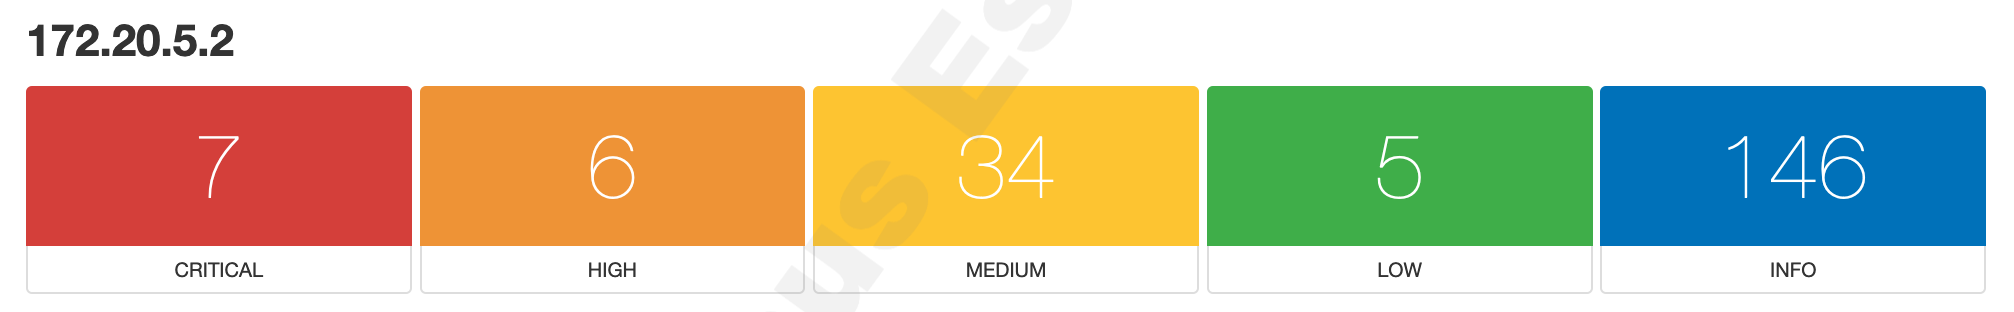
\includegraphics[width=1\linewidth]{img/vuln0.png}
 	\caption{Scan Summary}
\end{figure}

Nessus also has a \textbf{Remediations} list that has some advised actions that mitigate some vulnerabilities. For the vulnerabilities found, Nessus has some information such as it's \textbf{severity}, \textbf{how it can exploit it}, related \textbf{CVE's}, and more. Nessus also listed all the open ports, as well as all services running on them. There is also relevant information such as the target's \textbf{device typ}e and \textbf{OS}.
When comparing the results from our scan with the results of the automated one we found many similarities. In first place we investigated the ports where we struggled and found out that they either had a TLS service or a webserver tunning on them. Nessus managed to identify the services and even get the versions of TLS used. The only exception was port 8484, where Nessus wasn't able to find any information, hinting that it may be protected by a TCP Wrapper.
Nessus managed to extract information about TLS and SSL to an extent that we did not manage. The same happened with SSH, where Nessus we only got versions and hostkeys. Nessus even listed SSH Algorithms and supported languages.

Nessus managed to find \textbf{22 services} against the \textbf{15} we found. The OS detection made by Nessus returned the same result as we have with our search. With this comparison, the main conclusion we take is that with Nessus we manage to obtain more information compared to what we did before. Also the quality of the information obtained is superior, and quicker to obtain.

\subsection{Q3}

For this question we picked the following events from our IDS:\\

\begin{lstlisting}[basicstyle=\scriptsize]
    [**] [1:1418:11] SNMP request tcp [**]
    [Classification: Attempted Information Leak] [Priority: 2] 
    12/13-19:04:13.826861 172.20.5.1:1845 -> 172.20.5.2:161
    TCP TTL:64 TOS:0x0 ID:0 IpLen:20 DgmLen:48 DF
    ******S* Seq: 0xF614612C  Ack: 0x0  Win: 0x1000  TcpLen: 28
    TCP Options (4) => MSS: 1460 NOP NOP SackOK 
    [Xref => http://cve.mitre.org/cgi-bin/cvename.cgi?name=2002-0013]
    [Xref => http://cve.mitre.org/cgi-bin/cvename.cgi?name=2002-0012]
    [Xref => http://www.securityfocus.com/bid/4132]
    [Xref => http://www.securityfocus.com/bid/4089]
    [Xref => http://www.securityfocus.com/bid/4088]
\end{lstlisting}

By analysing the traffic captured by wireshark, we found 2 entries related to this event.

\begin{figure}[ht!]
 	\centering
 	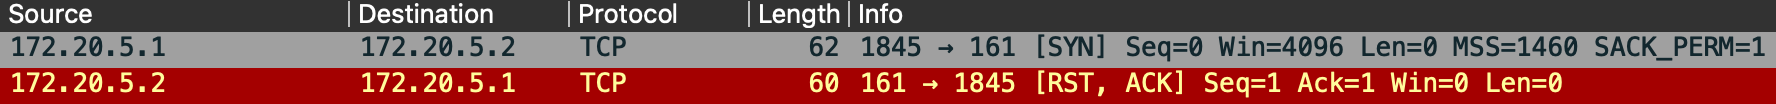
\includegraphics[width=1\linewidth]{img/wireshark1.png}
 	\caption{Packets in Wireshark}
\end{figure}

By analysing the packet sent to the target we noticed a \textbf{SYN flag}, which tells us that our host is trying to initiate connection with the target. But when we analyse the tcp segment that the target sends to our host, we noticed that in addition to the \textbf{ACK flag}, which isn't odd in this case, we have a \textbf{RST flag}. This may be caused by a  SYN packet trying to establish a connection to a port on which no process is listening. 

By searching the Snort Rules for this specific SID we found the \textbf{\href{https://www.snort.org/rule_docs/1-1418}{rule}} for this entry. The rule states that there was detected the presence of \textbf{SNMP} protocol, which has a lot of vulnerabilities used for \textbf{Denial of Service} and to \textbf{gain privileges}.

The CVE's related to this vulnerability are \textbf{CVE-2002-0013} and \textbf{CVE-2002-0012}. \\

\begin{lstlisting}[basicstyle=\scriptsize]
    [**] [1:249:8] DDOS mstream client to handler [**]
    [Classification: Attempted Denial of Service] [Priority: 2] 
    12/13-19:04:24.593643 172.20.5.1:9162 -> 172.20.5.2:15104
    TCP TTL:64 TOS:0x0 ID:0 IpLen:20 DgmLen:48 DF
    ******S* Seq: 0x1C77AAE7  Ack: 0x0  Win: 0x1000  TcpLen: 28
    TCP Options (4) => MSS: 1460 NOP NOP SackOK 
    [Xref => http://cve.mitre.org/cgi-bin/cvename.cgi?name=2000-0138]
    [Xref => http://www.whitehats.com/info/IDS111]
\end{lstlisting}

By analysing the traffic captured by wireshark, we found 7 entries related to this event, being the highlighted one that is registered in this event.

\begin{figure}[ht!]
 	\centering
 	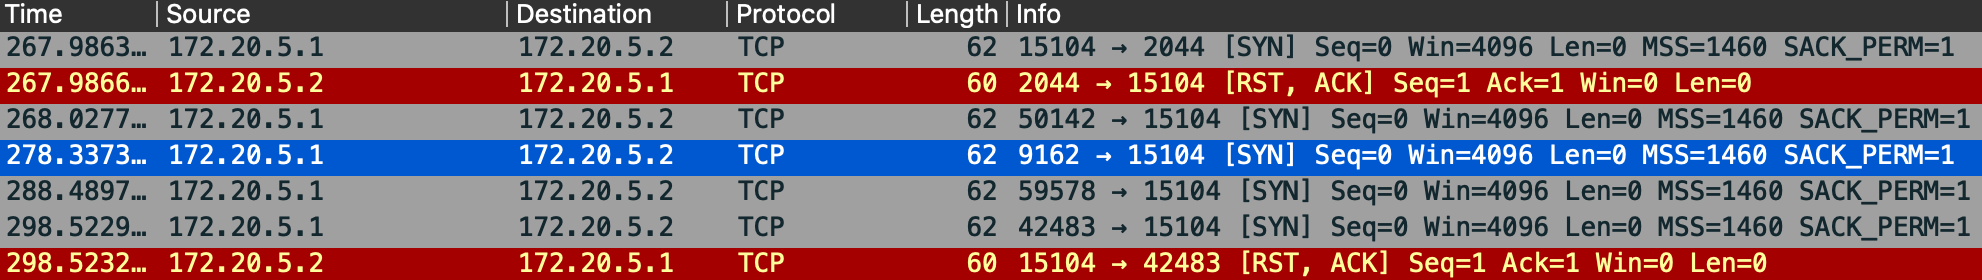
\includegraphics[width=1\linewidth]{img/wireshark2.png}
 	\caption{Packets in Wireshark}
\end{figure}

The first thing that we noticed was that the packet was similar to the one before, with the exception that this time, it was being sent periodically to the target, not getting a response sometimes. The packet that our host sent from port 50142 didn't get a response, and when the next packet was sent (from port 9162), the IDS registered the activity. 

By searching the Snort Rules for this specific SID we found the \textbf{\href{https://www.snort.org/rule_docs/1-249}{rule}} for this entry. The rule states that there was detected the presence of a distributed denial of service(DDOS) attack master, agent, or zombie.

The CVE related to this vulnerability is \textbf{CVE-2000-0138}. 

\subsection{Q4}

When analysing the output of the IDS and the output of Snort we noticed that some of the vulnerabilities listed on the IDS didn't show up on the vulnerability scanner. An example of this are the events listed in the previous question, which aren't listed on the report generated by Nessus. 

To discover what might be causing this we looked at what both IDS and vulnerability scanners do. The IDS basically monitors the network or system registering all kind of suspicious or malicious activity. Any intrusion activity or violation registered. The Scanner on the other hand, works in a different way, following a set of automated rules and redirecting it's focus on the go. For example, if the Scanner detects that the target system is a Windows host, it won't try to use vulnerabilities or exploits for Linux hosts. These kind of situations create some differences on what the IDS considers to be a threat and what a Scanner considers to be a threat.

\pagebreak

\subsection{Q5}

For this question we chose the following vulnerabilities:

\begin{itemize}
  \item 57608 - SMB Signing not required (Medium)
  \item 90192 - ManageEngine Desktop Central 8 / 9 < Build 91100 Multiple RCE (Critical)
  \item 134862 - Apache Tomcat AJP Connector Request Injection (Ghostcat) (High)
\end{itemize}

\begin{figure}[ht!]
 	\centering
 	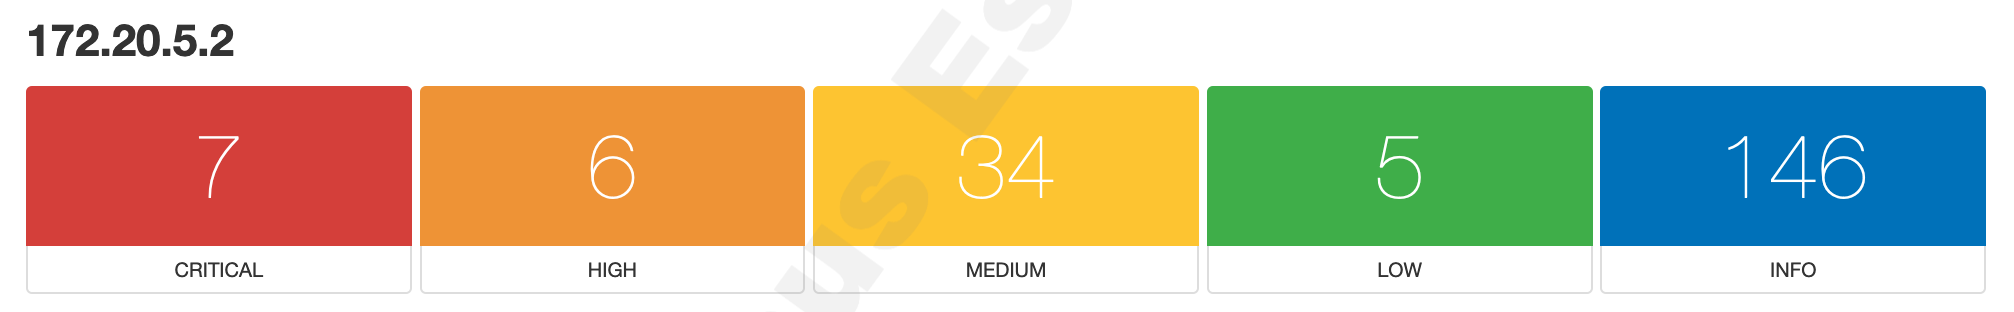
\includegraphics[width=1\linewidth]{img/vuln0.png}
 	\caption{Original Vulnerabilities}
\end{figure}

In order to resolve the first vulnerability we had to \textbf{enforce message signing in the host's configuration}. To do that we edited the windows registry key \textbf{HKLM\textbackslash System\textbackslash CurrentControlSet\textbackslash Services\textbackslash LanManServer\textbackslash Parameters\textbackslash \\RequireSecuritySignature} and set the flag to 1. What this does is requiring signatures for SMB communication. After this we rebooted the machine and performed a new scan, with the following results.

\begin{figure}[ht!]
 	\centering
 	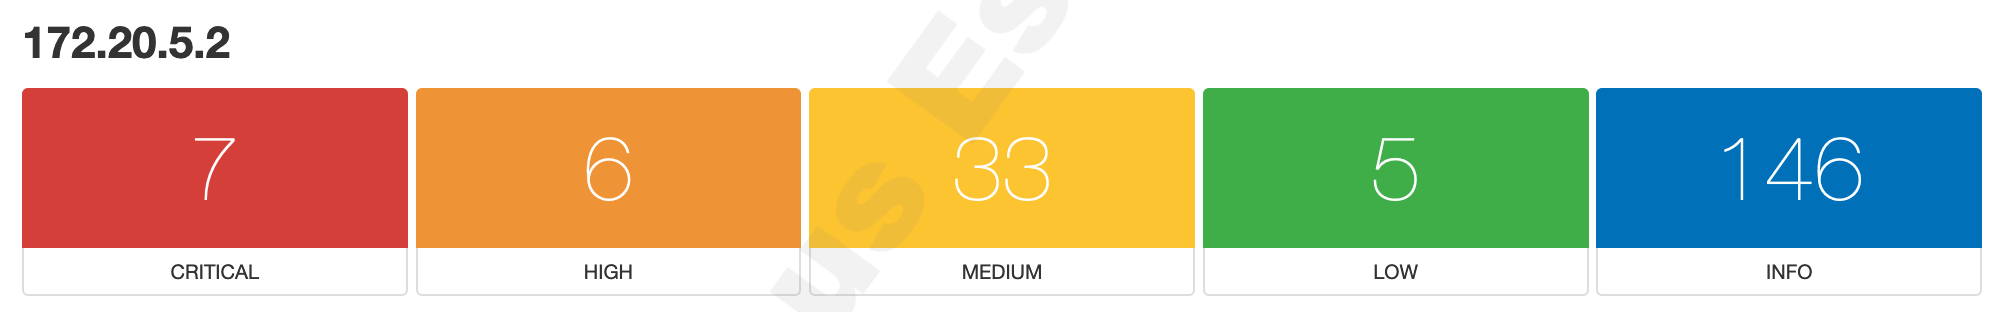
\includegraphics[width=1\linewidth]{img/vuln2.png}
 	\caption{Vulnerabilities after first fix}
\end{figure}

To fix the second vulnerability we updated \textbf{ManageEngine} to the latest version (10.0.650). The software update fixed the wanted vulnerability as we can see by running a new scan:

\begin{figure}[ht!]
 	\centering
 	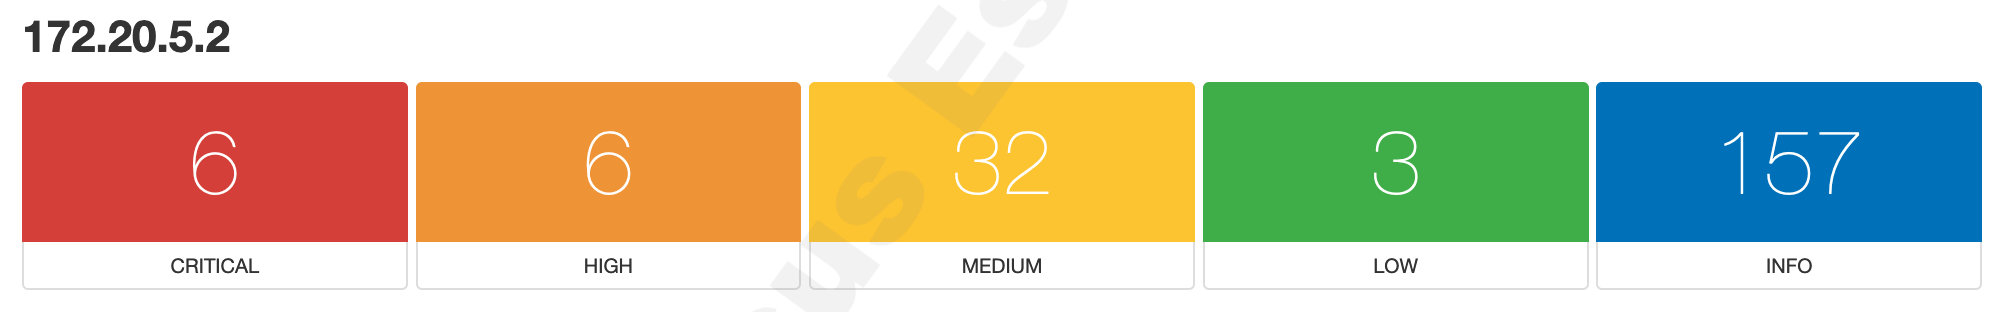
\includegraphics[width=1\linewidth]{img/vuln3.png}
 	\caption{Vulnerabilities after second fix}
\end{figure}

\pagebreak

Despite fixing the target vulnerability and some additional ones that were related with this same fix, there were also some new additions.

The last vulnerability we fixed was related to \textbf{Apache Tomcat}. The solution we applied was to update Tomcat to version 9.5.61. This fixed the vulnerability in question as we can see:

\begin{figure}[ht!]
 	\centering
 	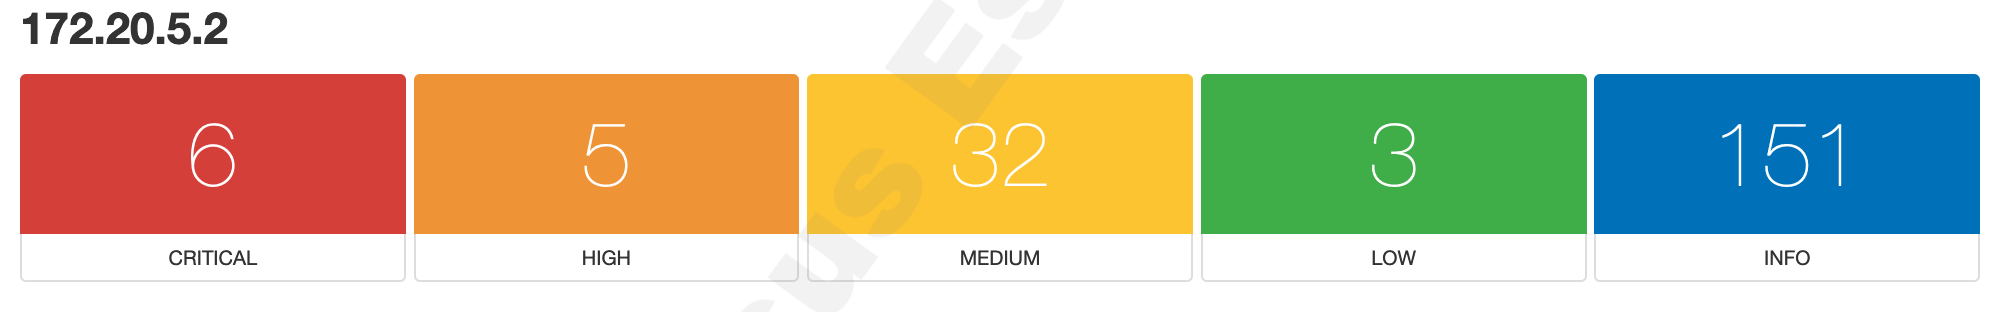
\includegraphics[width=1\linewidth]{img/vuln4.png}
 	\caption{Vulnerabilities after third fix}
\end{figure}

What we learned from this question is that with some minor system tweaks and some regular update cycles, we are able to mitigate a lot of security flaws on a system.

\pagebreak